\documentclass[letterpaper,12pt]{article}
\usepackage{tabularx} % extra features for tabular environment
\usepackage{amsmath}  % improve math presentation
\usepackage{commath}
\usepackage{graphicx} % takes care of graphic including machinery
\usepackage[margin=1in,letterpaper]{geometry} % decreases margins
\usepackage[final]{hyperref} % adds hyper links inside the generated pdf file
\usepackage[utf8]{inputenc}
\usepackage{authblk}
\usepackage{lipsum}
\usepackage{wrapfig}
\usepackage{float}
\usepackage[rightcaption]{sidecap}
\usepackage{array}
\usepackage{float}
%\usepackage[portuguese]{babel}
\usepackage{subcaption}
\usepackage{blindtext}
\usepackage{caption}
\usepackage{systeme}
%\graphicspath{ {./imagens/} }
\hypersetup{
    colorlinks=true,       % false: boxed links; true: colored links
    linkcolor=blue,        % color of internal links
    citecolor=blue,        % color of links to bibliography
    filecolor=magenta,     % color of file links
    urlcolor=blue
}
\usepackage{color}
\definecolor{light-gray}{gray}{0.95}
\usepackage{listings} 
\lstset{numbers=left, 
                numberstyle=\tiny, 
                breaklines=true,
                backgroundcolor=\color{light-gray},
                numbersep=5pt,
                xleftmargin=\parindent} 




%++++++++++++++++++++++++++++++++++++++++
 \title{
  Computational Physics \\
  \large 2º Trabalho Prático de Avaliação Continua \\
  Shooting Method and Fast Fourier Transform}
  
  
\author{João Maria Machado ,89132, PL4}

\begin{document}
\pagenumbering{Roman}

\maketitle


\newpage
\tableofcontents
\newpage

\section{Summary}
\pagenumbering{arabic}

In this report it will be made a computational analysis regarding a non-linear harmonic oscillator using a shooting method and the fast Fourier transform routine native to Matlab
\indent

After explaining the thought process behind the produced code an analysis over the obtained results will be made in order to verify that \textbf{there is accordance in between the different methods  when both are applied to the same situation}.


\section{Introduction} 
The studied physical system can be described by the following differential equation:  
\begin{equation}
m\frac{d^2y}{dt^2}+K(y+\alpha y^2)=\mu\left[ sen\left(\frac{dy}{dt}\right)\right]\frac{dy}{dt} \label{1}
\end{equation}

\indent 
As we can see the equation clearly describes a non-linear harmonic oscillator. More over the equation can be rearranged in order to make it easier to integrate. 
 
\begin{equation}
\frac{d^2y}{dt^2}=\frac{-K(y+\alpha y^2)+\mu\left[ sen\left(\frac{dy}{dt}\right)\right]\frac{dy}{dt}}{m} \label{2}
\end{equation}

\indent
This ordinary differential equation can be integrated using the ODE45 routine. However integrating is not enough! After the integration process the physical value of the amplitude must be attested (because it can be incorrect), and the integration process must be remade and adjusted accordingly. It is a boundary value problem and it will be solved using the \textbf{Shooting method}. In this case the shooting will be made in regards to \textbf{$\mu$} using two initial guesses (suggested in the test sheet) afterwards, the code will produce an \textbf{educated guess} and verify if the result produced by the guesses meet the established tolerance.


\section{Methods and Results}
\indent 
The first step done in order to start writing the code was to write the equations that describe the physical system in a way that can be easily written into Matlab.In the previous section there is already an equation \ref{2} that describes the oscillator's acceleration. After there is only need to substitute the derivatives by their physical meaning ($\frac{dy}{dt}=v$ and $\frac{d^2y}{dt^2}=\frac{dy}{dt}$, where v stands for velocity). \textbf{This system is the answer to question a) from part 1 }


\begin{equation}
  \systeme{
\frac{dv}{dt}=\frac{-K(y+\alpha y^2)+\mu\left[ sen\left(\frac{dy}{dt}\right)\right]\frac{dy}{dt}}{m}, 
\frac{dy}{dt}\,=v
  }
\label{3}
\end{equation}

\indent
After taking the necessary mathematical considerations the code can now be written. It is important to note that the main purpose of the code is not to only to integrate but to integrate 
while respecting the boundary conditions. As stated before, the code will "shoot" in respect to $\mu$ in order to satisfy the condition that the value of the amplitude is 2.15.

\newpage
\indent 
After implementing the code the following vector of values of $\mu$ was obtained (\textbf{the following row matrix is the answer to question b) from part 1}):

\begin{equation*}
\begin{bmatrix}
0.3500  &  0.4000  &  0.5074  &  0.4957 &   0.4965  &  0.4965  &  0.4965
\end{bmatrix}
\end{equation*}

\indent 
The last value is the value of $\mu$ that made the amplitude converge to the expected value. It should be noted that the value of $\mu$ as the number of integrations increases approaches \textbf{0.5} 


\indent
The next step in order to study the system is to analyse the trajectory in the phase space and find the period of the studied oscillator. The following graph, was obtained (the following set of figures contains the results found in order to\textbf{ answer question c) from part 1}) :

\begin{figure}[h]
  \centering
    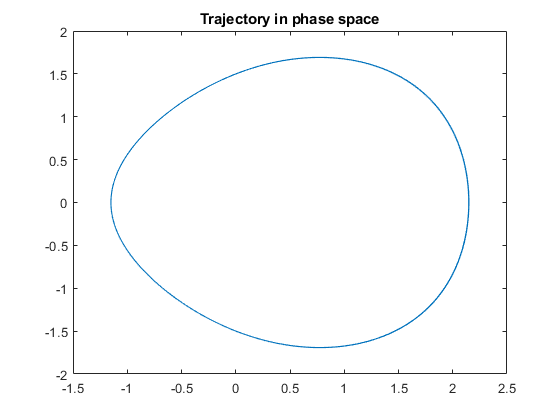
\includegraphics[scale=.7]{x.png}     
    \caption{Graph of Trajectory in phase space, as we can see the graph does not resemble an harmonic oscillator, due to the elliptical shape. The energy is being conserved}
\end{figure} 

\newpage
\indent
The value found for the period is \textbf{6.3619} (the value has no unit because no units are mentioned in the test sheet). This value can be confirmed for the integration done while analysing the graph of position over time:

\begin{figure}[h]
  \centering
    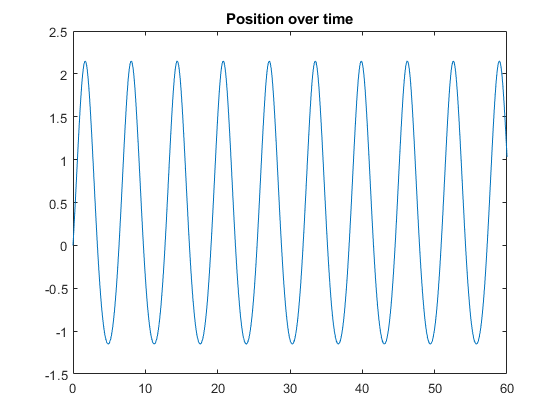
\includegraphics[scale=.7]{xt.png}     
    \caption{Graph of position over time, after taking a close look, it can be confirmed that value of period is close to the one computed previously, the graph confirms that the algorithm responsible for computing the period is correct}
\end{figure} 

\indent
Finally, the first part shall be concluded with an in depth analysis of the particular shooting method that was used. \textbf{The shooting and secant method} (\textbf{This part will answer question d) of part 1)}. As stated before the shooting method is used to ensure the accuracy of the integration and that it respects the boundary conditions. The method starts with 2 guesses given by the the programmer, afterwards it starts the integration process, when the first integration is completed it proceeds to access how accurate it was, this can be easily explained by the following expression:

\begin{equation*}
\abs{last.value.computed - boundary.value}<tolerance
\end{equation*}

where "\textbf{last.value.computed}" is the last computed value for a list of values, "\textbf{boundary.value}" is the of the boundary condition, the goal per say and "\textbf{tolerance}" is how the two compared values can differ.

\indent 
If the comparison step is successful the shooting is stopped, however if the estimate does not meet the boundary condition with the established tolerance the method restarts with \textbf{1 new guess and reuses one of the latest pair}. Unlike the first set these 2 new guesses are not random, one is reused and the other one can be calculated using the following formula:

   
\begin{equation*}
guess(3)=guess(2)+\frac{B-result(2)}{m}
\end{equation*}

\newpage
where B is the coordinated at origin and \textbf{m} is the slope of a particular linear equation. The slope can be calculated just like any slope but using the previous guesses and the results originated by them, as shown in the following expression:

\begin{equation*}
m=\frac{result(2)-result(1)}{guess(2)-guess(1)}
\end{equation*}
 
the \textbf{B} parameter can be computed by the following expression:

\begin{equation*}
B=result(2)-m \times guess(2)
\end{equation*}

\indent
After producing the 2 new educated guesses the program proceeds to check if the guesses produce an adequate result if so the program stops, otherwise the program does the algorithm explained before again.

\indent 

With these advancements made the analysis can now move on, by studying the system with regards to \textbf{Fourier analysis}. The first step in order to study the system is to produce the array of values of position and its length. Afterwards the vector of frequencies is ready to be calculated. The following formulas are used to allocate the vector of frequencies. 

\begin{equation*}
\Delta \omega= \frac{2 \pi}{N \Delta t} 
\end{equation*}

\begin{equation*}
\omega= \Delta \omega *[0:N-1]
\end{equation*}

Where N is the length (cardinality) of the array of the positions computed previously. $\Delta \omega$ is the step of the frequencies array and $\Delta t$ is the time step. After successfully calculating the frequencies the program is now ready to initiate the \textbf{FFT} routines. The following graph was obtained (\textbf{The next graph contains the answer the question e) and explain question g) of part 2}):

\begin{figure}[h]
  \centering
    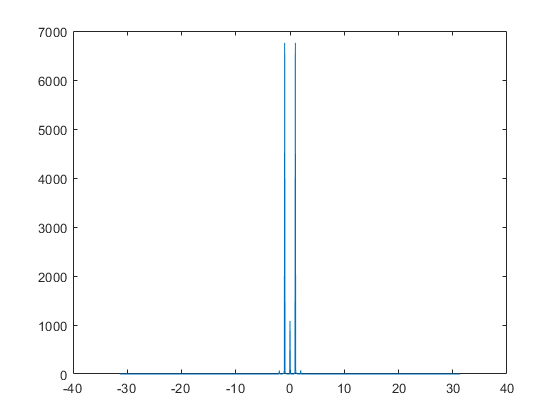
\includegraphics[scale=.5]{fft.png}     
    \caption{Fast Fourier transform (centred at 0) in which we can see the spectral density over frequencies, the graph suggests that  the movement seen i\textbf{s not typical of an harmonic oscillator, because it has more than two natural frequencies (peaks in the graph)}. }
\end{figure} 

\indent 
The next step is now to take the obtained results and select the values of spectral density and frequency bellow 10 and amplify them by a factor of 4. The produced graphs are the following (\textbf{this contains the answer to question f) from part 2}) :

\begin{figure}[h]
  \centering
    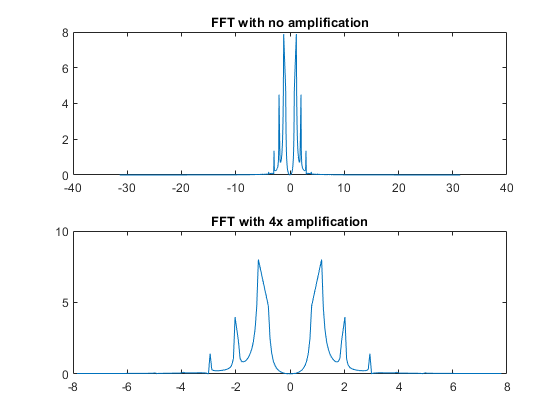
\includegraphics[scale=0.5]{amplificar.png}     
    \caption{Comparison between different FFT's  with different amplification, as the factor of amplification increases the peaks grow larger and more evident, \textbf{the oscillator is still not harmonic. There are more than two natural frequencies.} }
\end{figure} 

\indent 
One thing to note is the way that the spectral density is computed. The theoretical formula is simple (\textbf{the next equation is meant to respond to question g) from part 2}):


\begin{equation*}
dens=(\Delta t \times \abs{FFT})^2
\end{equation*}


\indent
Finally the last step is to check if the Fourier analysis is correct and apply it to the same context as before. A comparison will be made between the acceleration over time computed by two different methods. Via ODE45 and shooting method and the FFT route. However before presenting the results, the method used to derive the Fourier transform must be cited. The Fourier transform has a special rule when it comes to deriving it:

\begin{equation*}
F \left[ \frac{d^2f(t)}{dt^2} \right]= (i \omega)^2 F(\omega)
\end{equation*}

The logic of the question is simple, the current Fourier transform is made using the position over time if the transform is derived twice and then applied the IFFT (Inverse Fourier Transform) routine the following graphs can be obtained (\textbf{the following graph is meant to respond to question h) from part 2}):

\newpage
\begin{figure}[h]
  \centering
    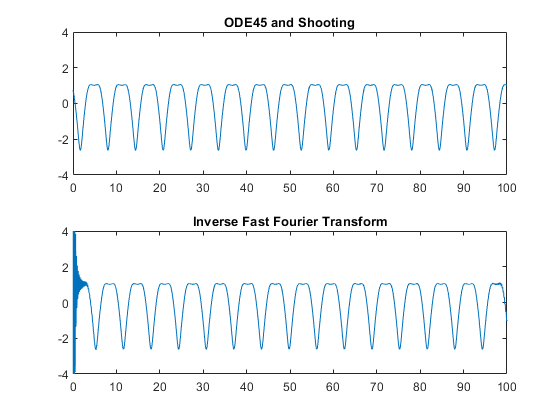
\includegraphics[scale=.7]{comp.png}     
    \caption{Comparison between the two graphs of acceleration over time, the different methods agree with each other however the FFT method presents some noise near t=0}
\end{figure} 

\section{Discussion and Conclusion}
The obtained results were precise and were coherent in their physical interpretation, there does not seem to appear any significant error, however minor errors can be lowered in the program if the time step is decreased thus making the integration more precise and making the sampling larger (in the case of the FFT). 

\indent
As stated before the results are coherent with the physics thus one could say that the goal was achieved. Mainhe


\end{document}

